\begin{center}
  \Large
  \textbf{BIOGRAFI PENULIS}
\end{center}

\addcontentsline{toc}{chapter}{BIOGRAFI PENULIS}

\vspace{2ex}

\begin{wrapfigure}{L}{0.3\textwidth}
  \centering
  \vspace{-3ex}
  % Ubah file gambar berikut dengan file foto dari mahasiswa
  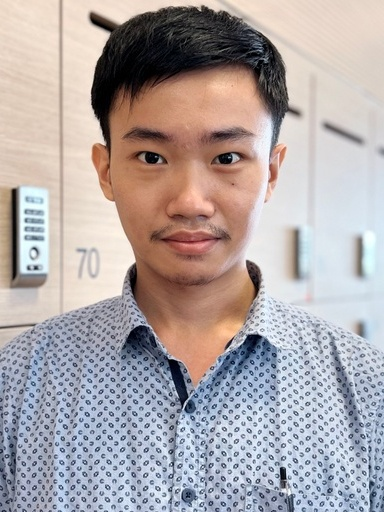
\includegraphics[width=0.3\textwidth]{gambar/me.jpg}
  \vspace{-4ex}
\end{wrapfigure}

% Ubah kalimat berikut dengan biografi dari mahasiswa
\name{} adalah seorang penulis dan pengembang perangkat lunak yang lahir di Surabaya pada tanggal 8 Desember 2001. Penulis menyelesaikan pendidikannya di Institut Teknologi Sepuluh Nopember, dengan mengambil jurusan Teknik Komputer.
Sejak awal masa studinya, penulis telah menunjukkan minat dan keahlian yang besar dalam bidang pengembangan perangkat lunak. Penulis aktif terlibat dalam berbagai kegiatan di kampus, termasuk menjadi anggota panitpenulis dalam acara MAGE 6 dan MAGE 7, yang merupakan acara besar dalam dunpenulis komputer dan teknologi.
Ketertarikan penulis terutama terfokus pada pengembangan backend dan aplikasi. Penulis memiliki pemahaman yang mendalam tentang berbagai bahasa pemrograman dan kerangka kerja yang digunakan dalam pengembangan perangkat lunak modern. Keahliannya dalam backend development memungkinkan penulis untuk mengembangkan sistem yang kuat dan efisien.
Selain itu, penulis juga memiliki ketertarikan khusus dalam topik blockchain. Dalam tugas akhirnya, penulis memilih untuk fokus pada penelitian dan pengembangan blockchain, sebuah teknologi yang memiliki potensi untuk merevolusi berbagai sektor, termasuk keuangan dan logistik.
Dalam perjalanan penulisannya, penulis telah menghasilkan berbagai artikel dan tulisan teknis terkait dengan bidang pengembangan perangkat lunak. Penulis memiliki kemampuan komunikasi yang baik dan mampu menyampaikan ide-idenya dengan jelas dan terstruktur.
Sebagai seorang yang berdedikasi dan bersemangat, penulis terus mengembangkan keterampilan dan pengetahuannya dalam industri teknologi yang terus berkembang. Penulis selalu berusaha untuk mengikuti perkembangan terbaru dalam dunpenulis pengembangan perangkat lunak dan mengaplikasikannya dalam pekerjaannya.
Jika Anda ingin menghubungi penulis, Anda dapat menghubungi melalui email di me@aaronct.dev. Penulis sangat terbuka untuk kolaborasi dan diskusi terkait dengan pengembangan perangkat lunak dan topik terkait lainnya.
